\documentclass[journal]{IEEEtran}

\usepackage{blindtext}
\usepackage{graphicx}
\usepackage{cite}
\usepackage[utf8x]{inputenc}
\usepackage[slovene,english]{babel}  
\usepackage{url}

\hyphenation{op-tical net-works semi-conduc-tor}
\begin{document}
\title{IMapBooks - Automatic Question Response Grading}
\author{Tilen Tomakić\\tt5157@student.uni-lj.si\\https://github.com/TilenTomakic/IMapBooks-AQRG}%
\maketitle

%  Abstract -  summary of problem and contribution
\begin{abstract}	
  Dokument opisuje raziskavo metod mapiranja, ekstrakcije informacij in uporabe korpusa za točkovanje pravilnosti odgovorov na vprašanja iz podane zgodbe. Raziskani so bili tri modeli. Od najpreprostejšega do naprednejšega.
\end{abstract}

\begin{IEEEkeywords}
NLP, IMapBook, SAG
\end{IEEEkeywords}

\IEEEpeerreviewmaketitle

% Introduction - problem motivation and background
\section{Uvod}
Cilj dokumenta je raziskati tehnike ovrednotenja pravilnosti odgovorov. Pri ovrednotenju je na voljo množica že ovrednotenih odgovorov na enaka vprašanja in izvirno besedilo. Vsi pravilni odgovori so snovani le na podlagi izvornega besedila.

Algoritem zaznave pravilih in napačnih odgovorov lahko prevedemo na širše probleme, kot so zaznava lažnih novic.\\

Raziskava je bila osnovana na podatkovni množici vprašanj in odgovor iz IMapBook (https://www.imapbook.com/) vira. V množici, sta dva učitelja ovrednotila odgovore učencev na temo prebrane zgodbe. Odgovor je ovrednoten s 0, 0,5 ali 1 točko.\\

Opisani so tri pristopi reševanja problema. Modeli A, B in C. Enako kot učitelja modeli ovrednotijo odgovore s točkami 0, 0,5 ali 1.

%  Related work - relevant literature overview
\section{Podobna dela}
Podobna dela se delijo v več skupin oz. kombinacije~\cite{adhya2016automated}.

- Mapiranje: ATM, C-Rater, ...
% Ideja mapiranja temelji na primerjanju če odgovor vsebuje določene zveze. Lahko primerjamo na nivoju stavkov, besed ali n-gramov.
% Primer: ~\cite{wang2018identifying}
- Ekstrakcija informacij
- Uporaba korpusa
- Strojno učenje\\

V angleščini problemski domeni rečejo "Short Answer Grading (SAG)". SAG se ukvarja z ocenjevanjem krajših odgovorov (2-3 stavki).


%  Methods - used methods and techniques
\section{Uporabljene metode}
\subsection{Model A}
Model A se že v začetku odloči za en odgovor iz množice vseh pravilnih. Odloči se na podlagi kriterija najpopolnejšega odgovora. Odgovor, ki ima večje število besed se smatra kot najpopolnejši.
Izbran odgovor je uporabljen za ocenjevaje drugih. Bolj sta si odgovora podobna večja je verjetnost, da je ocenjevan odgovor pravilen. Pri primerjanju je odgovor razbit na korene besed.

\subsection{Model B}
Model B je podoben modelu A, vendar se ne odloči se za statičen odgovor na začetku. Pravilnost odgovora testira nad celotno znano množico odgovorov.

Ker ima B model na voljo celotno množico odgovor, je bil uporabljena K-means metoda gručenja (nimam še rezultatov, implementacija v izdelavi).

% bag of words

\subsection{Model C}
Pri modelu C so vsakemu odgovoru dodane sopomenke. 

Uporaba C-net API-ja (nimam še rezultatov, implementacija v izdelavi).

% Results - results description
\section{Rezultati}
Uspešnosti modelov je vidna na tabeli~\ref{t:mod}.

\begin{table}[]
	\begin{tabular}{l|l|l|l|}
		\cline{2-4}
		                            & Model A          & Model B          & Model C          \\ \hline
		\multicolumn{1}{|l|}{Vprašanje 1} & \textbf{?\%} & \textbf{?\%} & \textbf{?\%} \\ \hline
		\multicolumn{1}{|l|}{Vprašanje 2} & \textbf{?\%} & \textbf{?\%} & \textbf{?\%} \\ \hline
		\multicolumn{1}{|l|}{Vprašanje 3} & \textbf{?\%} & \textbf{?\%} & \textbf{?\%} \\ \hline
		\multicolumn{1}{|l|}{Vprašanje 4} & \textbf{?\%} & \textbf{?\%} & \textbf{?\%} \\ \hline
		\multicolumn{1}{|l|}{Vprašanje 5} & \textbf{?\%} & \textbf{?\%} & \textbf{?\%} \\ \hline
		\multicolumn{1}{|l|}{Skupaj} & \textbf{38.47\%} & \textbf{63.65\%} & \textbf{68.82\%} \\ \hline
	\end{tabular}
	\caption{Uspešnost modelov}
	\label{t:mod}
\end{table}

\begin{figure}[!t]
	\centering
	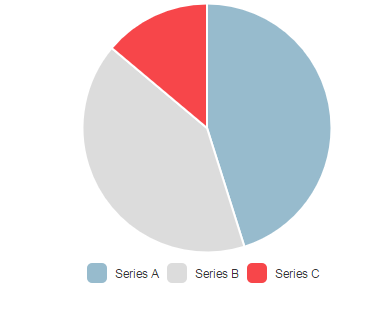
\includegraphics[width=2.5in]{chart}
	\caption{TODO}
	\label{sl:ma}
\end{figure}

% Discussion - results comparison and evaluation
%\section{Discussion}

\section{Zaključek}
Že v sami IMapBook množici, se dva ocenjevalca pri vseh odgovorih nista strinjala o njihovi oceni. Pri ocenjevanju je računalniški algoritem lahko le tako dober kot je človek. Če se niti človek ne more strinjati o oceni, je težko pričakovati, da bo algoritem opravil boljše.\\

Izvorna koda modelov in strežnik za preizkus je na voljo na git repozitoriju: https://github.com/TilenTomakic/IMapBooks-AQRG

\ifCLASSOPTIONcaptionsoff
  \newpage
\fi

% literature (use BibTeX)
\bibliographystyle{IEEEtran}
\bibliography{literatura}

\end{document}
